\section{Tracks}
\label{sec:ch6_tracks}

\subsection{Reconstruction}

A track is reconstructed by fitting the trajectory of a charged particle to hits in the ID.
Its momentum and charge are determined from the curvature in the magnetic field, while its position near the beam line is used to assign it to a production vertex.
Track reconstruction is performed in the following stages~\cite{ATLAS2017DenseTracking}:
\begin{enumerate}
    \item \textbf{Space-point formation.} Signals in neighbouring channels of a silicon sensor are grouped into clusters. The coordinates provided by Pixel clusters and SCT clusters are converted into three-dimensional space points.
    \item \textbf{Seeding and track finding.} Combinations of space points are used to form track seeds. These seeds are extended through the silicon layers with a combinatorial Kalman filter, which is used to refine the track parameters.
    \item \textbf{Ambiguity resolution.} Track candidates are ranked using their fit quality, momentum and hit variables. Meawhile, candidates that share the same clusters are marked as "shared hits". Candidatges fail the track-quality requirement are then rejected to suppress duplicate and fake tracks.
    \item \textbf{TRT extension.} Tracks are extended with additional TRT hits. The extended track is retained if its quality score is higher than that of the original track reconstructed using only pixel and SCT hits.
\end{enumerate}

\subsection{Track parameters and quality}

The fitted trajectory is described by five parameters, as illustrated in Figure~\ref{fig:ch6_track_parameters}:
\begin{itemize}
    \item $d_0$: distance in the $x-y$ plane between the beam line and the perigee point, defined as the point on the track closest to the beam line.
    \item $z_0$: the $z$ coordinate of the perigee point relative to the reference plane at $z=0$.
    \item $\phi$ and $\theta$: the azimuthal and polar angles of the momentum, respectively.
    \item $q/p$: the electric charge divided by the momentum magnitude.
\end{itemize}

Two quantities are used to test whether a track is consistent with production at the primary vertex~\cite{ATLAS2021MuonID}:
\begin{itemize}
    \item \textbf{Transverse impact-parameter significance}, $d_0/\sigma_{d_0}$: the transverse distance from the beam line in units of its uncertainty $\sigma_{d_0}$.
    \item \textbf{Projected longitudinal distance}, $\Delta z_0\sin\theta=(z_0-z_{\mathrm{PV}})\sin\theta$: the longitudinal distance between the track perigee and the primary vertex. Here, $z_{\mathrm{PV}}$ is the $z$ coordinate of the primary vertex.
\end{itemize}

Small absolute values of both quantities suggest that the track is from the primary vertex.
A large longitudinal distance can also indicate a track from another $pp$ collision.
Prompt electron and muon candidates are therefore selected by requiring small values of both quantities, and displaced candidates with large values can originate from a separate decay vertex, for example from a $b$- or $c$-hadron decay.

\begin{figure}[htbp]
    \centering
    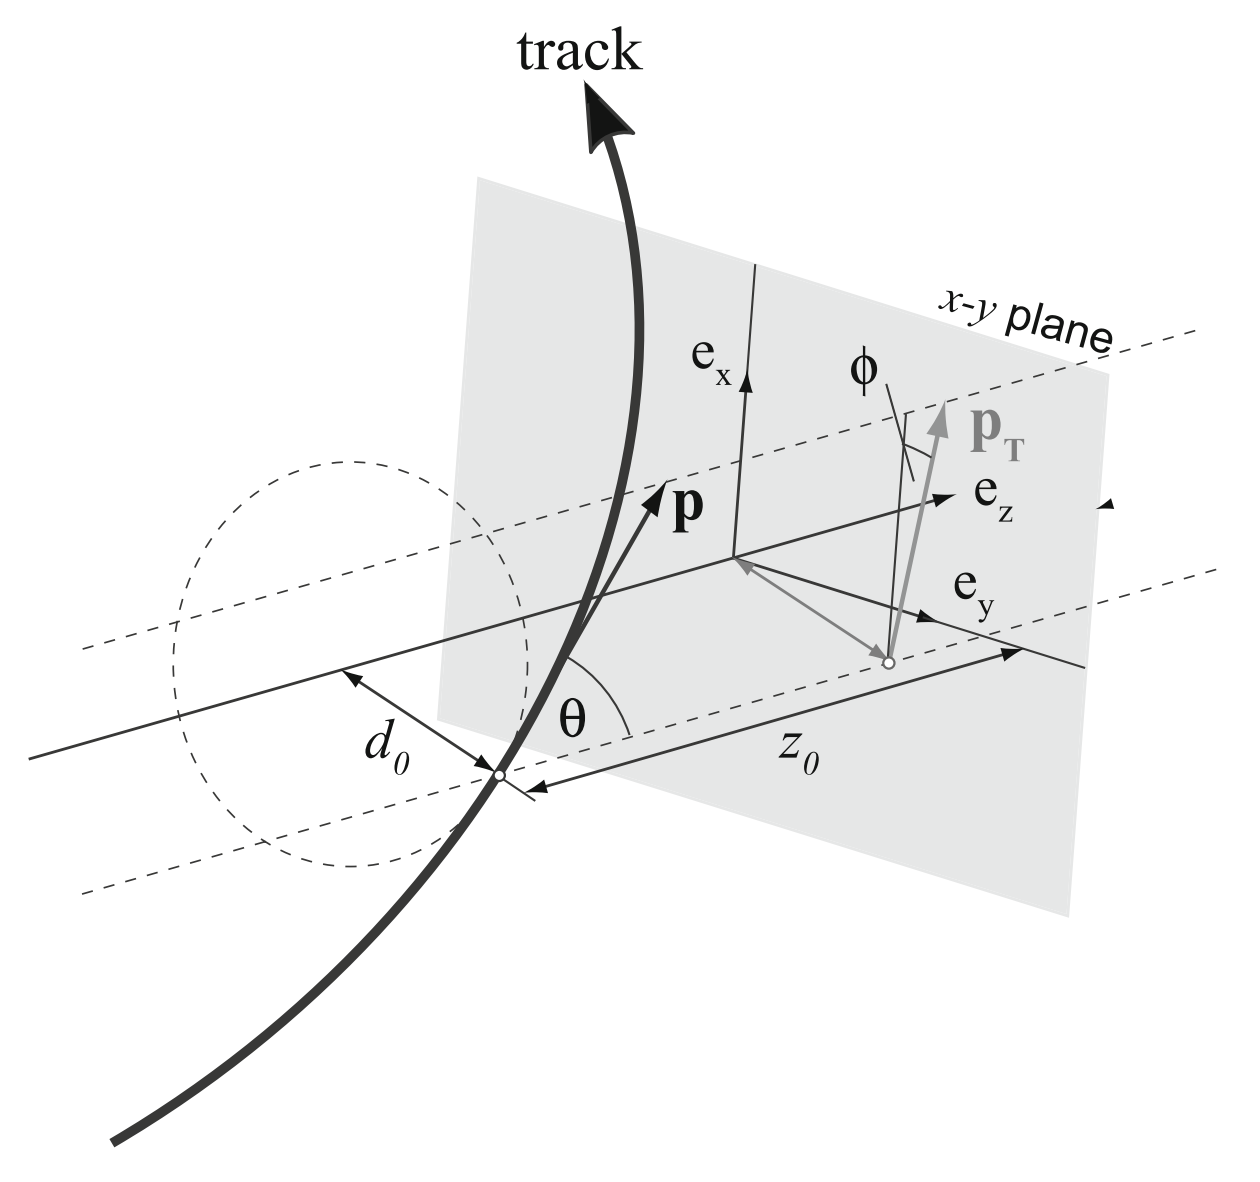
\includegraphics[width=0.58\textwidth]{Figs/CH6/track_parameters.png}
    \caption[Geometry of the Track parameters]{Geometry of the Track parameters. The grey plane represents the reference $z=0$ plane~\cite{ATLAS2025SoftwareComputing}.}
    \label{fig:ch6_track_parameters}
\end{figure}
